% secciones/implementacion_hive.tex

\section{Implementación en Apache Hive}

\subsection{Creación de la base de datos y tablas}

Se creó la base de datos \texttt{retail} en el metastore de Hive y se definieron las
cinco tablas obligatorias del benchmark \tpcds{} como tablas externas, de modo que los
datos almacenados en HDFS no se eliminen al ejecutar \texttt{DROP TABLE}.

\begin{lstlisting}[style=hiveql, caption={DDL: creación de base de datos y tabla customer}]
CREATE DATABASE IF NOT EXISTS retail;
USE retail;

CREATE EXTERNAL TABLE IF NOT EXISTS customer (
    c_customer_sk    BIGINT,
    c_first_name     STRING,
    c_last_name      STRING,
    c_email_address  STRING,
    c_birth_year     INT,
    c_birth_country  STRING
)
ROW FORMAT DELIMITED
FIELDS TERMINATED BY '|'
STORED AS TEXTFILE
LOCATION '/user/hadoop/tpcds/customer/';
\end{lstlisting}

Las tablas \texttt{item}, \texttt{store}, \texttt{date\_dim} y \texttt{store\_sales}
siguen el mismo patrón con sus respectivos esquemas TPC-DS.

\begin{figure}[H]
    \centering
    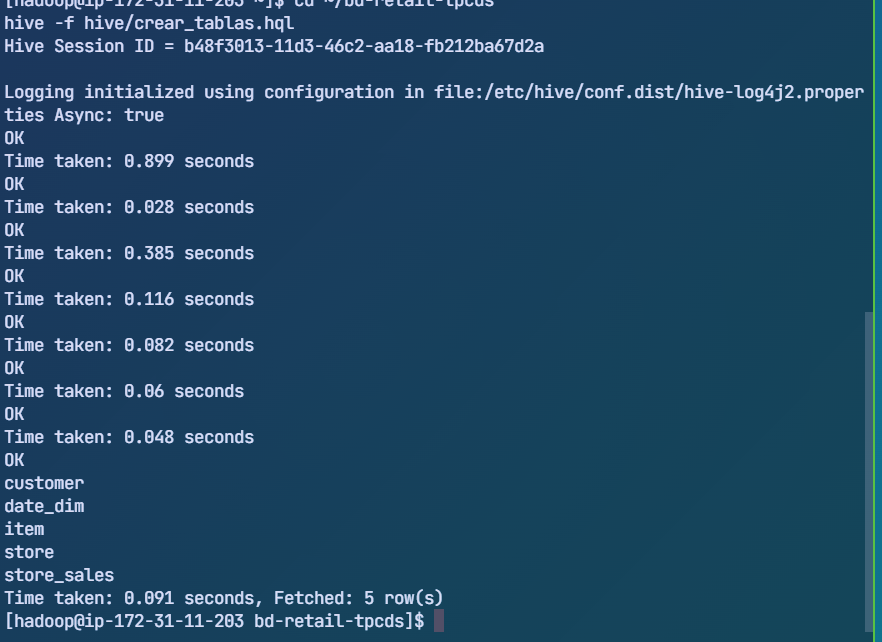
\includegraphics[width=0.85\textwidth]{figuras/hive_show_tables.png}
    \caption{Resultado de \texttt{SHOW TABLES} en Hive tras la creación del esquema retail.}
\end{figure}

\subsection{Consultas analíticas}

A continuación se presentan las consultas HiveQL implementadas sobre el Data Warehouse retail.

\subsubsection{Top 20 clientes con mayor número de compras}

\begin{lstlisting}[style=hiveql, caption={Q1: Top 20 clientes por número de compras}]
SELECT
    c.c_customer_sk,
    c.c_first_name,
    c.c_last_name,
    COUNT(ss.ss_ticket_number) AS total_compras
FROM store_sales ss
JOIN customer c ON ss.ss_customer_sk = c.c_customer_sk
GROUP BY c.c_customer_sk, c.c_first_name, c.c_last_name
ORDER BY total_compras DESC
LIMIT 20;
\end{lstlisting}

\begin{figure}[H]
    \centering
    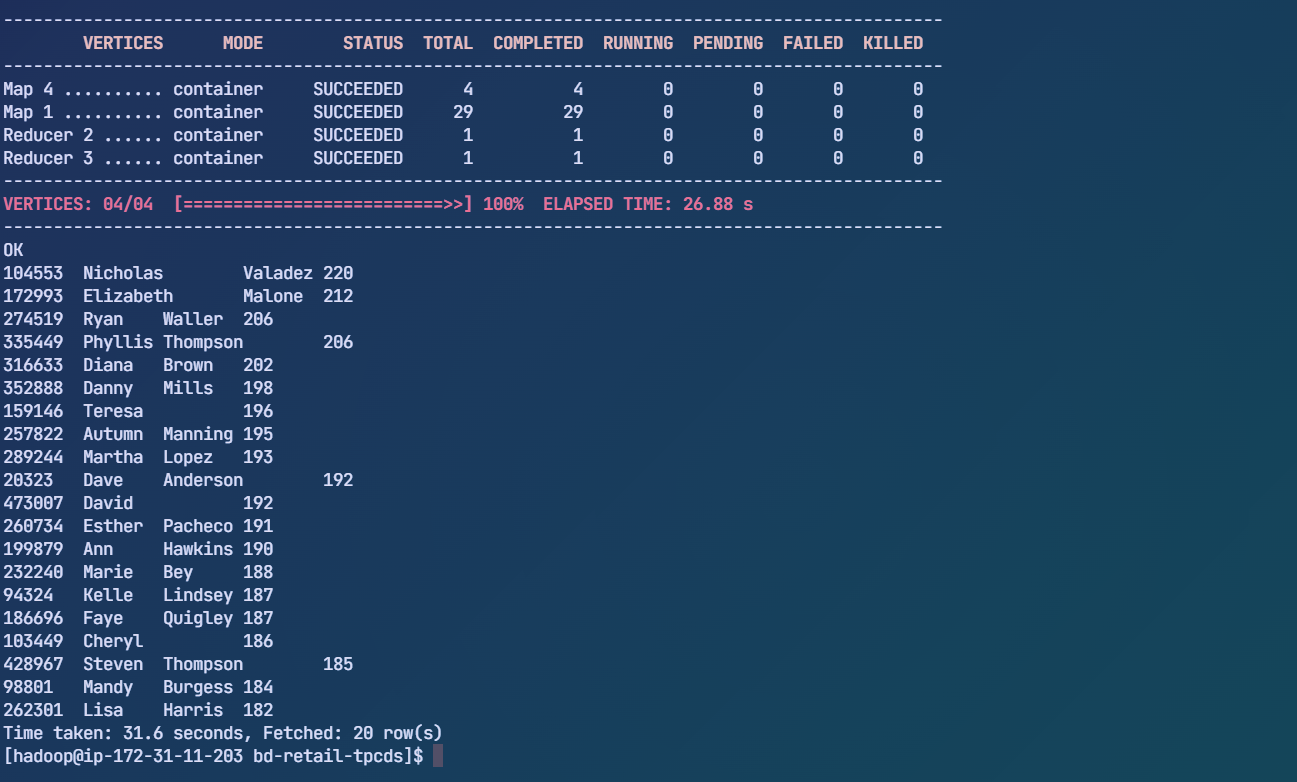
\includegraphics[width=0.85\textwidth]{figuras/hive_q1_resultado.png}
    \caption{Resultado de Q1 en Hive: top 20 clientes por número de compras.}
\end{figure}

\subsubsection{Ventas por tienda}

\begin{lstlisting}[style=hiveql, caption={Q2: Ventas totales agrupadas por tienda}]
SELECT
    s.s_store_name,
    COUNT(ss.ss_ticket_number)  AS total_transacciones,
    SUM(ss.ss_net_paid)         AS ingresos_totales,
    AVG(ss.ss_net_paid)         AS ingreso_promedio
FROM store_sales ss
JOIN store s ON ss.ss_store_sk = s.s_store_sk
GROUP BY s.s_store_sk, s.s_store_name
ORDER BY ingresos_totales DESC;
\end{lstlisting}

\begin{figure}[H]
    \centering
    \includegraphics[width=0.85\textwidth]{figuras/hive_q2_resultado.png}
    \caption{Resultado de Q2 en Hive: ventas por tienda.}
\end{figure}

\subsubsection{Ventas por mes}

\begin{lstlisting}[style=hiveql, caption={Q3: Ventas agrupadas por año y mes}]
SELECT
    d.d_year  AS anio,
    d.d_moy   AS mes,
    COUNT(ss.ss_ticket_number) AS total_transacciones,
    SUM(ss.ss_net_paid)        AS ingresos_totales
FROM store_sales ss
JOIN date_dim d ON ss.ss_sold_date_sk = d.d_date_sk
GROUP BY d.d_year, d.d_moy
ORDER BY d.d_year, d.d_moy;
\end{lstlisting}

\begin{figure}[H]
    \centering
    \includegraphics[width=0.85\textwidth]{figuras/hive_q3_resultado.png}
    \caption{Resultado de Q3 en Hive: ventas por mes.}
\end{figure}

\subsubsection{Ventas por día de la semana}

\begin{lstlisting}[style=hiveql, caption={Q4: Ventas agrupadas por día de la semana}]
SELECT
    d.d_day_name               AS dia_semana,
    d.d_dow                    AS numero_dia,
    COUNT(ss.ss_ticket_number) AS total_transacciones,
    SUM(ss.ss_net_paid)        AS ingresos_totales
FROM store_sales ss
JOIN date_dim d ON ss.ss_sold_date_sk = d.d_date_sk
GROUP BY d.d_day_name, d.d_dow
ORDER BY d.d_dow;
\end{lstlisting}

\begin{figure}[H]
    \centering
    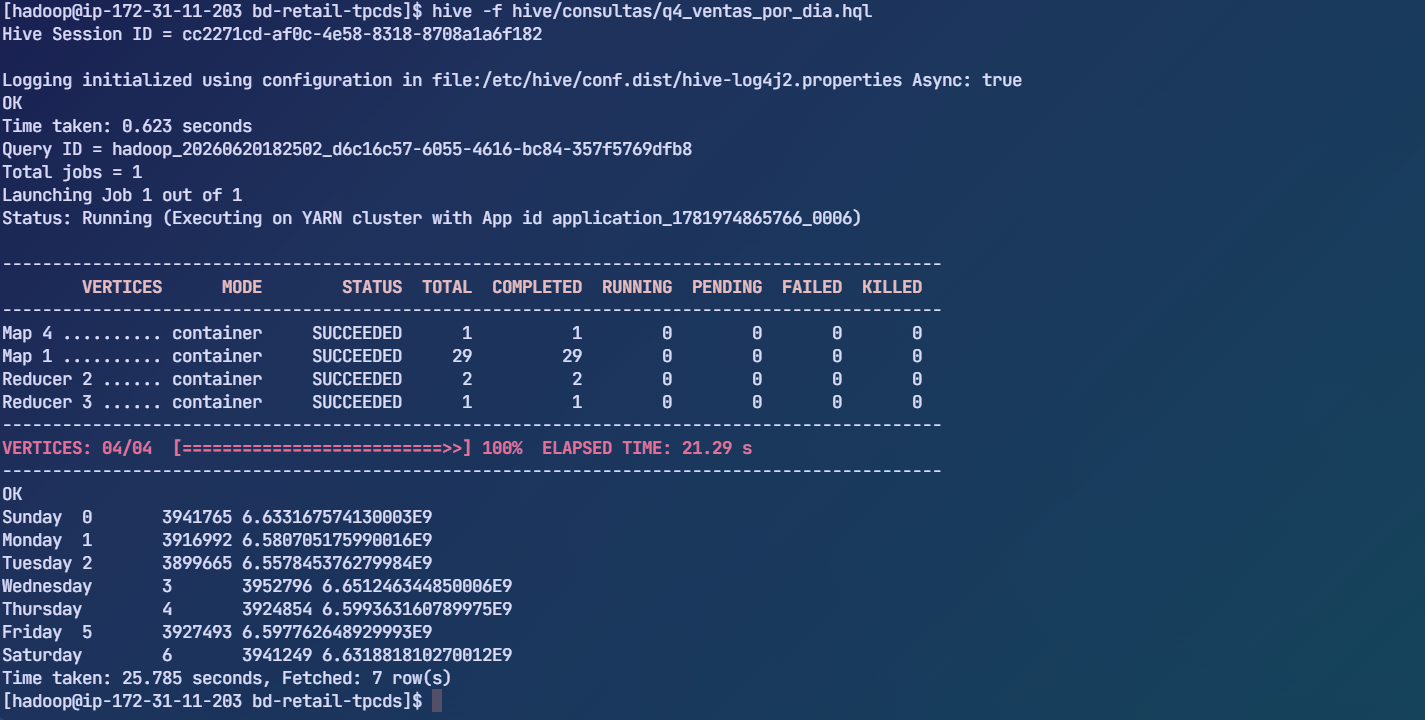
\includegraphics[width=0.85\textwidth]{figuras/hive_q4_resultado.png}
    \caption{Resultado de Q4 en Hive: ventas por día de la semana.}
\end{figure}

\subsubsection{Top productos por tienda}

\begin{lstlisting}[style=hiveql, caption={Q5: Top 5 productos por tienda usando QUALIFY}]
SELECT
    s.s_store_name,
    i.i_product_name,
    SUM(ss.ss_quantity)  AS unidades_vendidas,
    SUM(ss.ss_net_paid)  AS ingresos_totales
FROM store_sales ss
JOIN store s ON ss.ss_store_sk = s.s_store_sk
JOIN item  i ON ss.ss_item_sk  = i.i_item_sk
GROUP BY s.s_store_name, i.i_product_name
QUALIFY ROW_NUMBER() OVER (
    PARTITION BY s.s_store_name
    ORDER BY SUM(ss.ss_quantity) DESC
) <= 5
ORDER BY s.s_store_name, unidades_vendidas DESC;
\end{lstlisting}

\begin{figure}[H]
    \centering
    \includegraphics[width=0.85\textwidth]{figuras/hive_q5_resultado.png}
    \caption{Resultado de Q5 en Hive: top productos por tienda.}
\end{figure}

\subsubsection{Ticket promedio por cliente}

\begin{lstlisting}[style=hiveql, caption={Q6: Ticket promedio de compra por cliente}]
SELECT
    c.c_first_name,
    c.c_last_name,
    COUNT(DISTINCT ss.ss_ticket_number)                        AS total_tickets,
    SUM(ss.ss_net_paid)                                       AS gasto_total,
    SUM(ss.ss_net_paid) / COUNT(DISTINCT ss.ss_ticket_number) AS ticket_promedio
FROM store_sales ss
JOIN customer c ON ss.ss_customer_sk = c.c_customer_sk
GROUP BY c.c_customer_sk, c.c_first_name, c.c_last_name
ORDER BY ticket_promedio DESC
LIMIT 50;
\end{lstlisting}

\begin{figure}[H]
    \centering
    \includegraphics[width=0.85\textwidth]{figuras/hive_q6_resultado.png}
    \caption{Resultado de Q6 en Hive: ticket promedio por cliente.}
\end{figure}

\subsubsection{Productos con mayor ingreso generado}

\begin{lstlisting}[style=hiveql, caption={Q7: Productos con mayor ingreso total}]
SELECT
    i.i_product_name,
    i.i_category,
    i.i_brand,
    SUM(ss.ss_quantity)  AS unidades_vendidas,
    SUM(ss.ss_net_paid)  AS ingresos_totales
FROM store_sales ss
JOIN item i ON ss.ss_item_sk = i.i_item_sk
GROUP BY i.i_item_sk, i.i_product_name, i.i_category, i.i_brand
ORDER BY ingresos_totales DESC
LIMIT 20;
\end{lstlisting}

\begin{figure}[H]
    \centering
    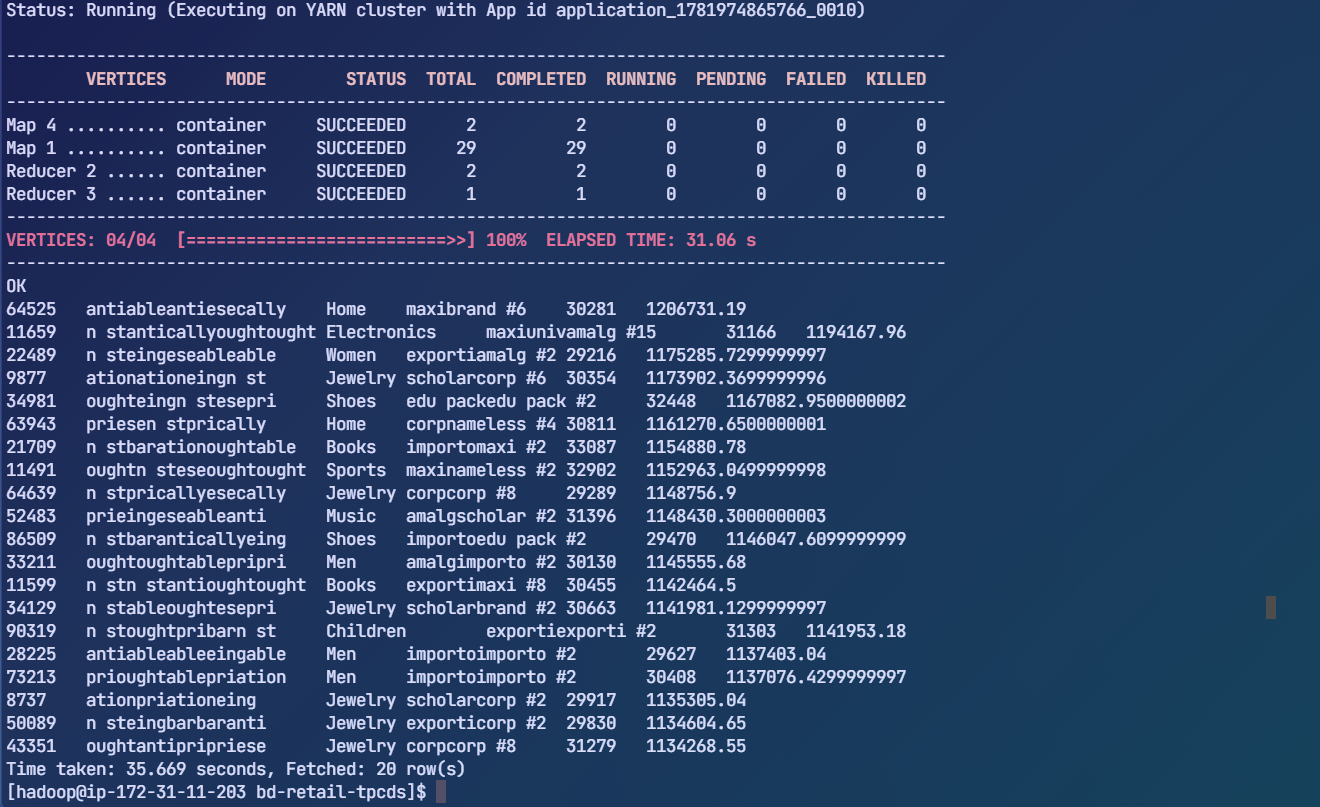
\includegraphics[width=0.85\textwidth]{figuras/hive_q7_resultado.png}
    \caption{Resultado de Q7 en Hive: productos con mayor ingreso.}
\end{figure}

\subsubsection{Top clientes por gasto total}

\begin{lstlisting}[style=hiveql, caption={Q8: Top 20 clientes por gasto total}]
SELECT
    c.c_first_name,
    c.c_last_name,
    c.c_email_address,
    SUM(ss.ss_net_paid)                 AS gasto_total,
    COUNT(DISTINCT ss.ss_ticket_number) AS total_tickets
FROM store_sales ss
JOIN customer c ON ss.ss_customer_sk = c.c_customer_sk
GROUP BY c.c_customer_sk, c.c_first_name, c.c_last_name, c.c_email_address
ORDER BY gasto_total DESC
LIMIT 20;
\end{lstlisting}

\begin{figure}[H]
    \centering
    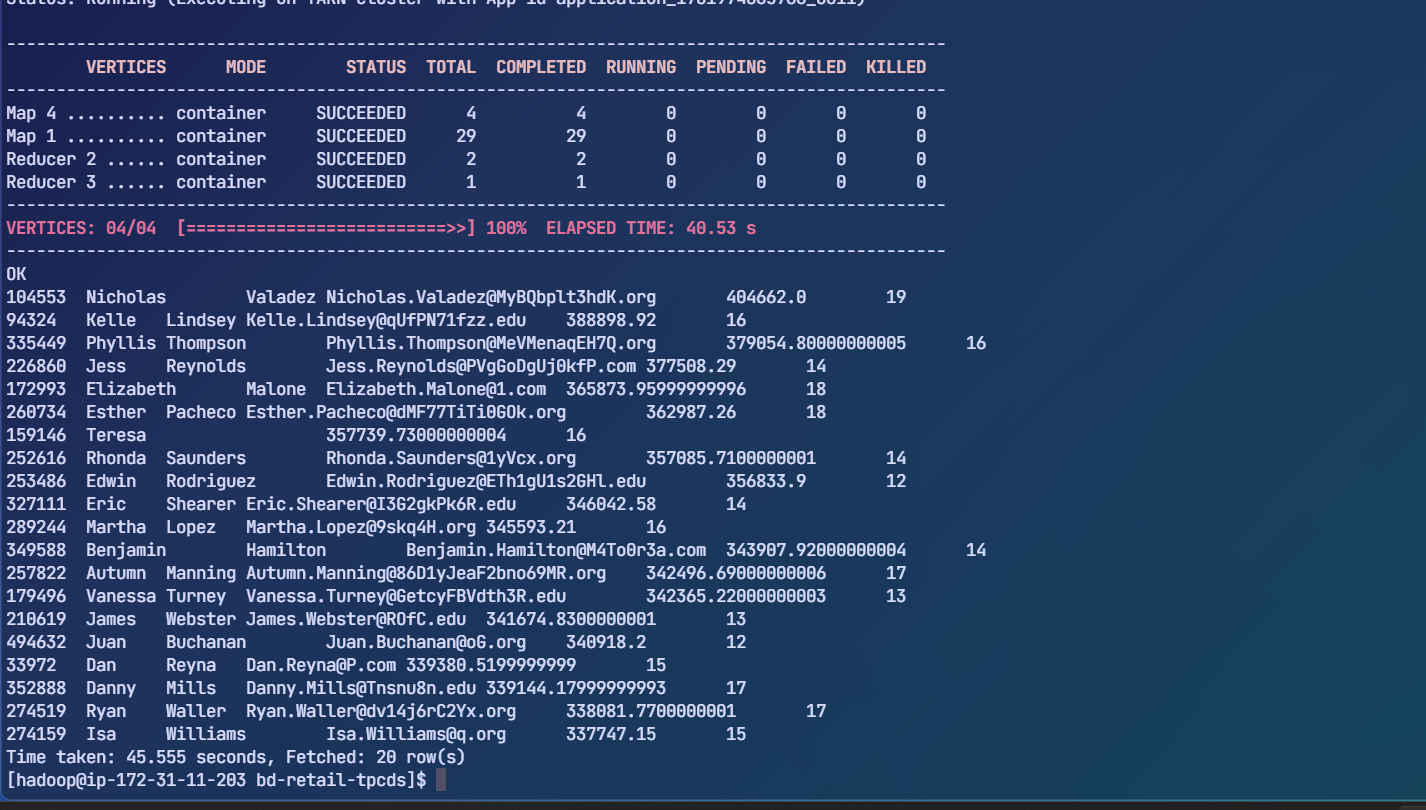
\includegraphics[width=0.85\textwidth]{figuras/hive_q8_resultado.png}
    \caption{Resultado de Q8 en Hive: top clientes por gasto total.}
\end{figure}

\subsubsection{Ranking mensual de ventas}

\begin{lstlisting}[style=hiveql, caption={Q9: Ranking mensual de tiendas por ingresos}]
SELECT
    d.d_year            AS anio,
    d.d_moy             AS mes,
    s.s_store_name,
    SUM(ss.ss_net_paid) AS ingresos_totales,
    RANK() OVER (
        PARTITION BY d.d_year, d.d_moy
        ORDER BY SUM(ss.ss_net_paid) DESC
    ) AS ranking
FROM store_sales ss
JOIN date_dim d ON ss.ss_sold_date_sk = d.d_date_sk
JOIN store    s ON ss.ss_store_sk     = s.s_store_sk
GROUP BY d.d_year, d.d_moy, s.s_store_name
ORDER BY d.d_year, d.d_moy, ranking;
\end{lstlisting}

\begin{figure}[H]
    \centering
    \includegraphics[width=0.85\textwidth]{figuras/hive_q9_resultado.png}
    \caption{Resultado de Q9 en Hive: ranking mensual de ventas por tienda.}
\end{figure}
